In Kangaroo certain computations need to be performed in the background periodically.  Android OS provides a nice solution for this requirement with the Service class. Each class that extends Service can perform computations without the need of a foreground user interface. The only mandatory element that needs to be overwritten is the onCreate() method. This method is called when a new instance of the class is created. Once the service sleeps in memory until it is called, unless the phone runs out of RAM. in that case the object is terminated, so has no control over its lifecycle. When a service is called with the corresponding intent its onStart() method is called.\\\\
\begin{figure}[h!]
\centering
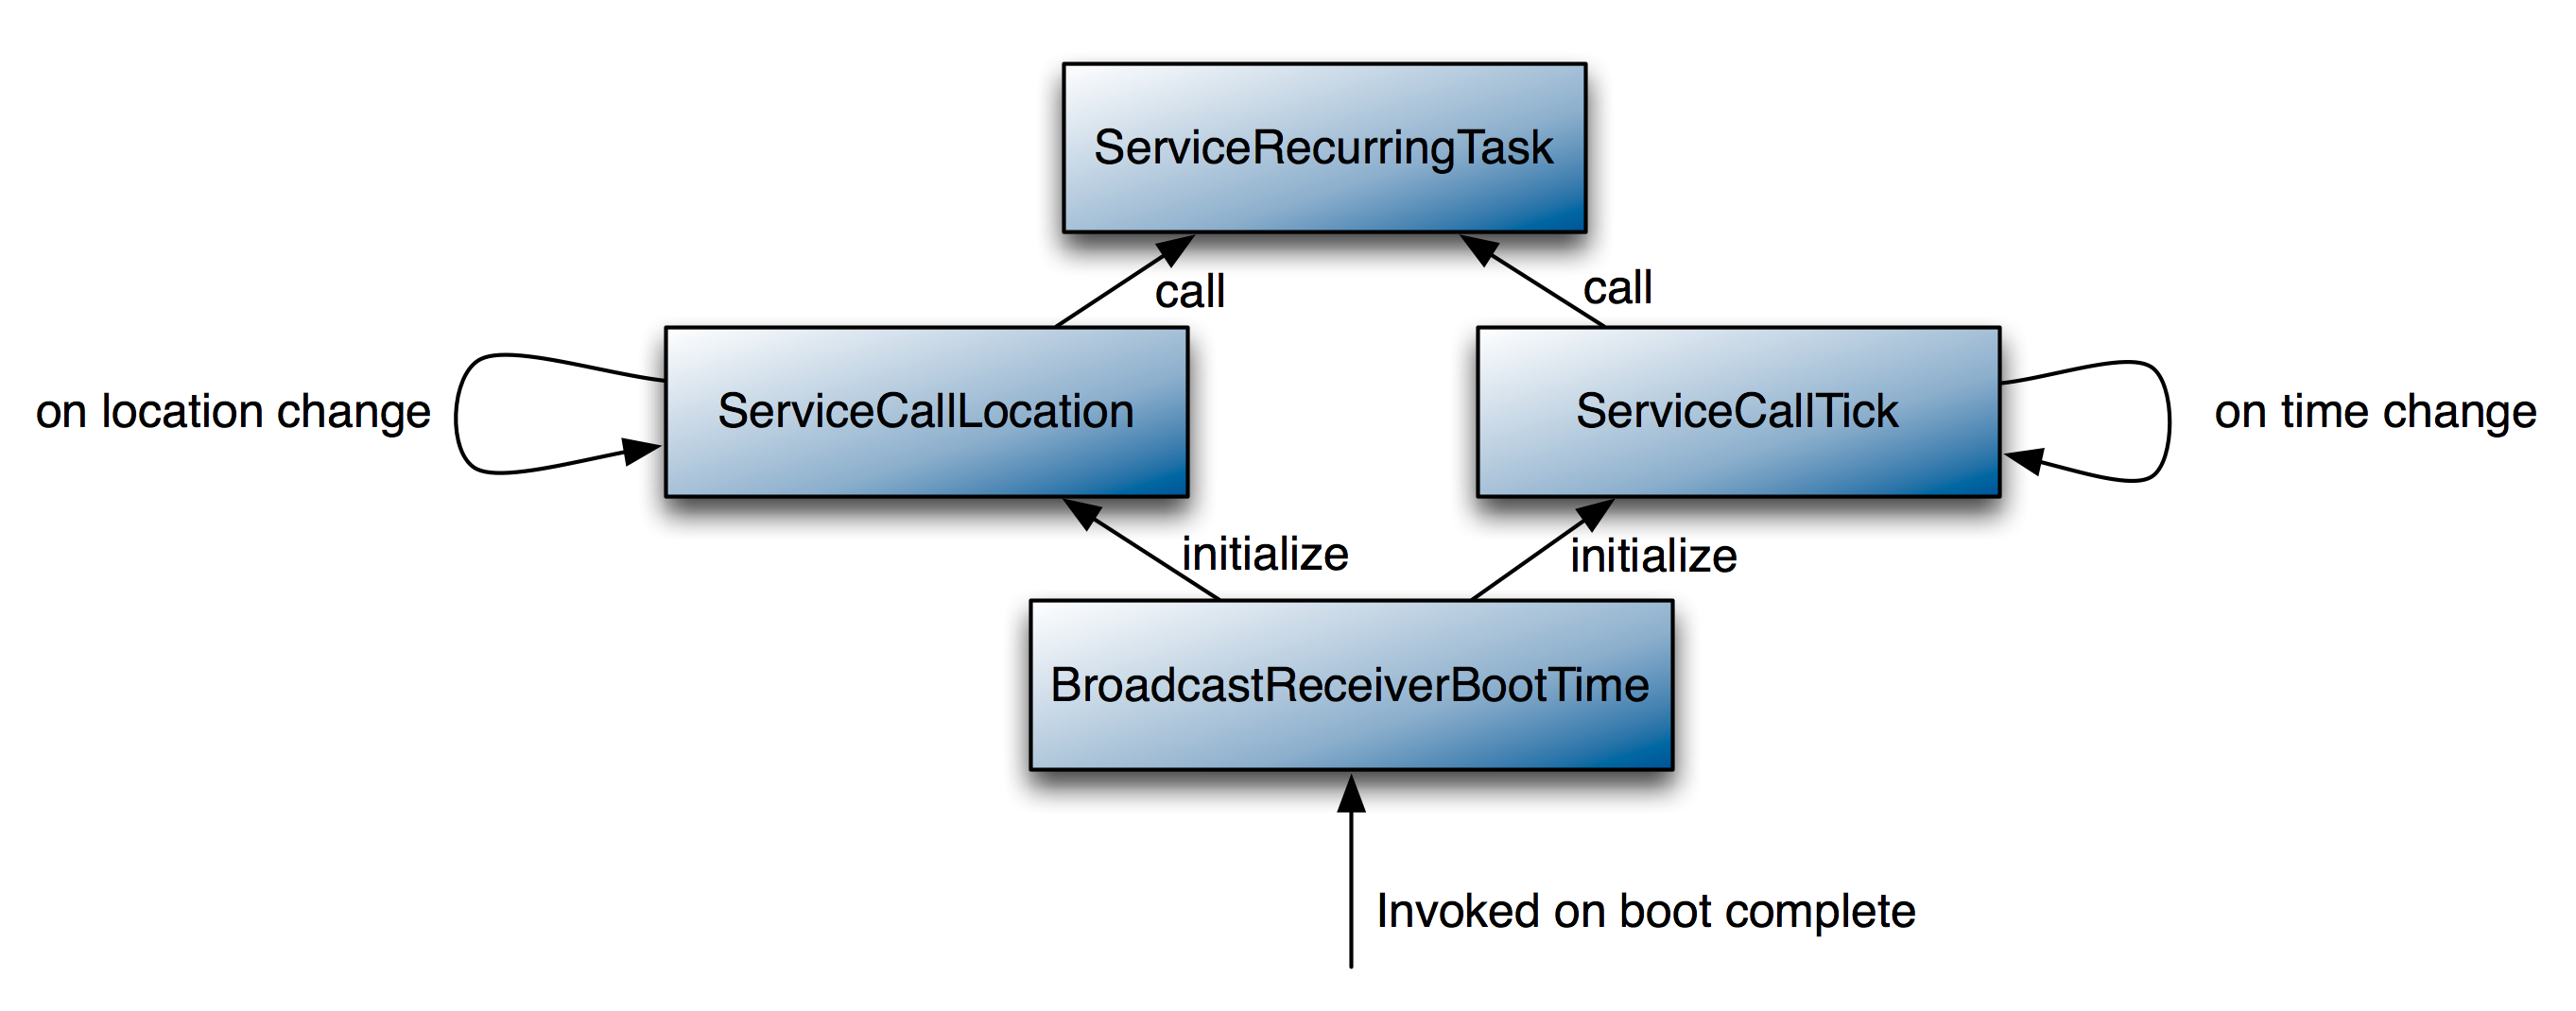
\includegraphics[width=14cm]{pics/background1.png}
\caption{Interaction of the background task classes}
\label{background1}
\end{figure}  
The services implemented in Kangaroo are located in the com.kangaroo.system package and shown in figure \ref{background1}. The BroadcastReceiverBootTime implements a BroadcastReceiver that listens to the boot-time broadcast from the OS. The receiver can be registered for a certain broadcast in the AndroidManifest.xml.
\begin{verbatim}  
  <intent-filter>	  
      <action android:name=''android.intent.action.BOOT_COMPLETED'' />
  </intent-filter>
\end{verbatim}
Once the phone has started correctly the code in the onReceive() method is executed. Here the services ServiceCallLocation and ServiceCallTick are started. ServiceCallLocation registers itself with the Android LocationManager. The service is then called every time the location of the phone has changed more than x meters. 
ServiceCallTick registers  with the AlarmManager. It is called every time a certain amount of time has passed.
Both of the services execute one task in their onStart() method: they call the ServiceRecurringTask with a corresponding intent:
 \begin{verbatim}  
Intent callIntent = new Intent(ServiceCallTick.this, ServiceRecurringTask.class);
callIntent.putExtra("isLocation", false);
startService(callIntent);
\end{verbatim}
In the ServiceRecurringTask the commands shown in figure \ref{background2} are executed.
\begin{itemize}
\item First the semaphore is checked. Since location and time updates occur independently of each other, the semaphore prevents the ServiceRecurringTask from being called multiple times simultaneously. 
\item Then a new thread is created. Since the service is executed in the main tread of the application, performing extensive calculations without a separate thread could cause the GUI to lag. 
\item Next a wake-lock on the CPU is obtained to prevent Android from putting the process to sleep. It is very important to release the wake-lock as soon as possible, since the inability of the CPU to go to a low power state drains the phone battery quickly. 
\item After that an instance of the com.kangaroo.ActiveDayPlan is acquired and the methods to check consistency and reachability of the day plan are called. If the plan is not consistent or a event can not be reached in time, a notification to the user is generated. (see chapter \ref{sec:user_interface}) 
\item Then the semaphore and the wake-lock are released and the thread terminates.
\end{itemize}
\begin{figure}[h!]
\centering
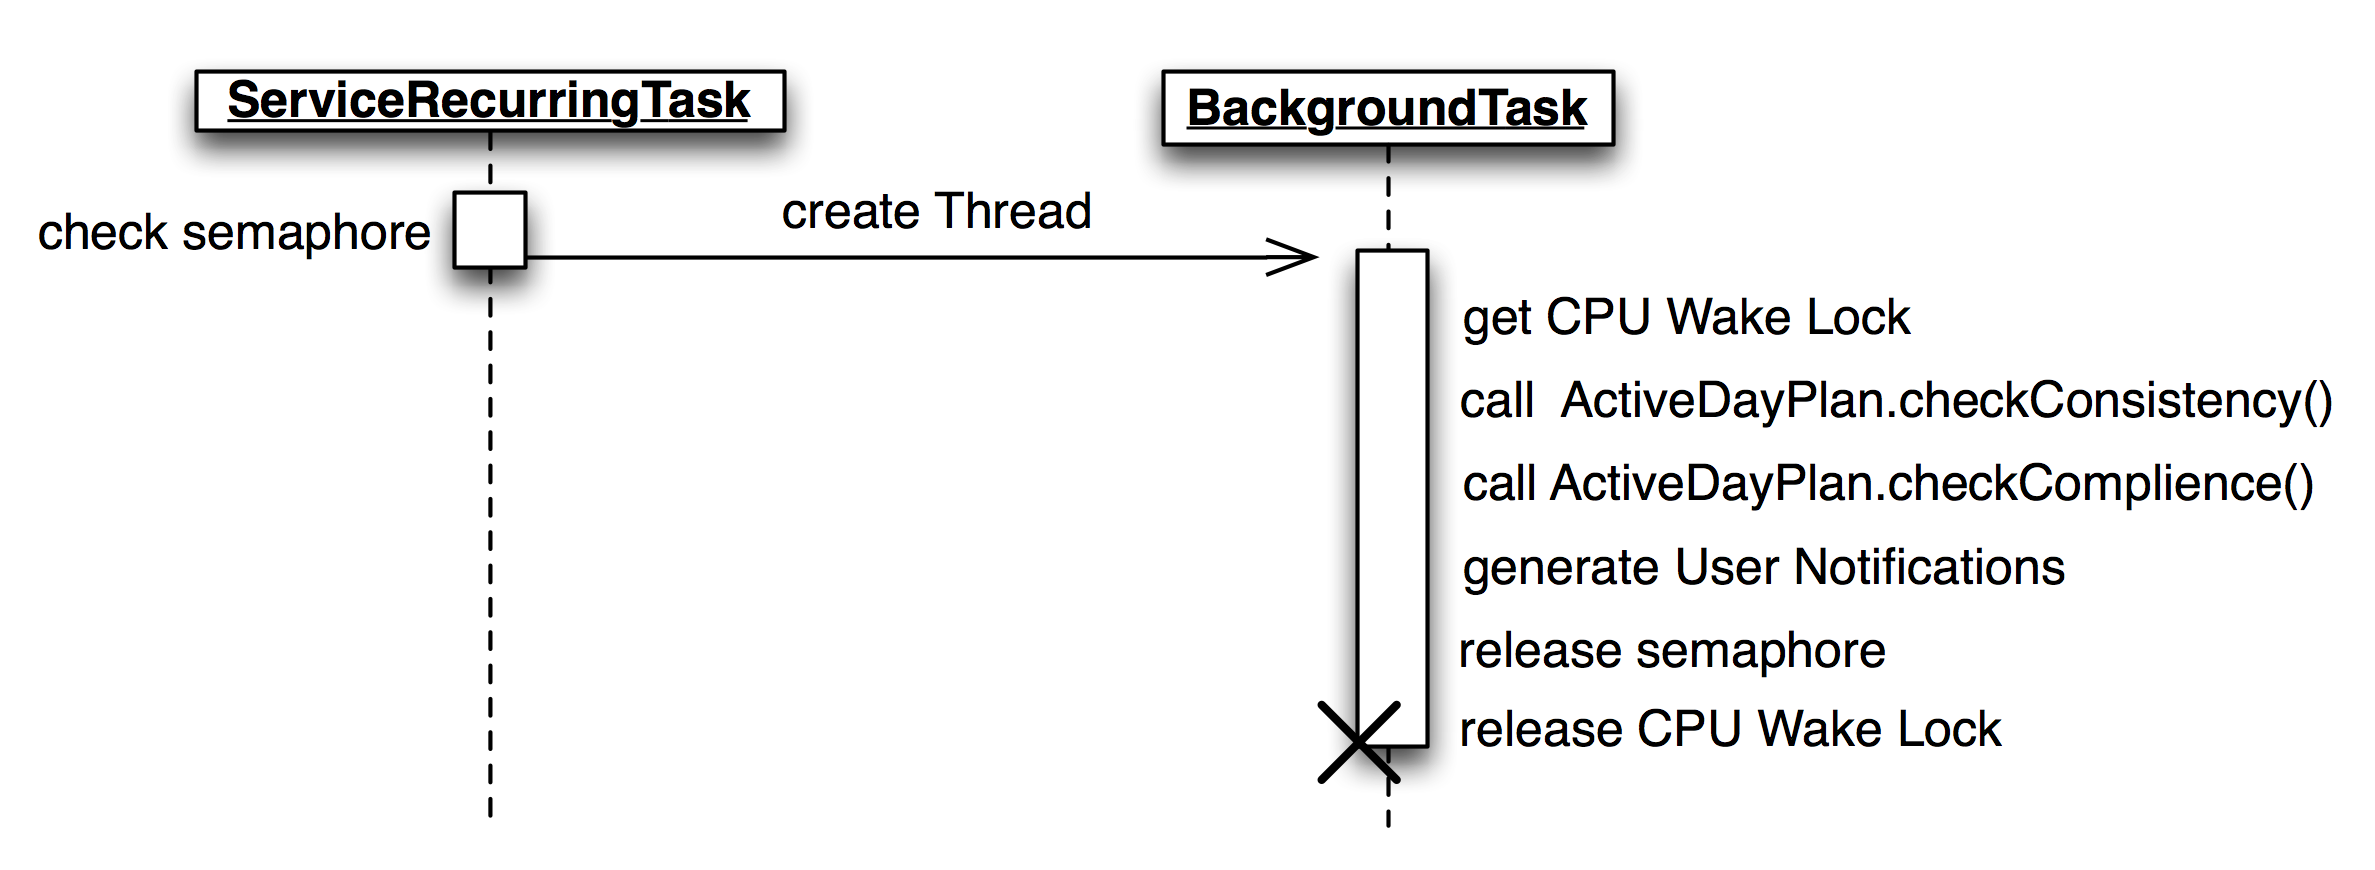
\includegraphics[width=14cm]{pics/background2.png}
\caption{Sequence diagram of the background task}
\label{background2}
\end{figure}  
